
%--------------------------------------
%ELECTROTECHNIQUE - SCHEMA DE LIAISON A LA TERRE
%--------------------------------------

%utiliser les environnement \begin{comment} \end{comment} pour mettre en commentaire le préambule une fois la programmation appelée dans le document maître (!ne pas oublier de mettre en commentaire \end{document}!)

\begin{comment}

\documentclass[a4paper, 11pt, twoside, fleqn]{memoir}

\usepackage{AOCDTF}

\marqueurchapitre

%lien d'édition des figures Tikz sur le site mathcha.io (rajouter le lien d'une modification effectuée sur la figure tikz avec le nom du modificateur car il n'y a qu'un lien par compte)

%lien éditeur Bruno Douchy : https://www.mathcha.io/editor/4zmjBS4GfLpHL48e8frKpd9lfP0E5lDHXe51Ln

%--------------------------------------
%corps du document
%--------------------------------------

\begin{document} %corps du document
	\openleft %début de chapitre à gauche

\end{comment}

\begin{figure}
\caption{Répartition des volumes dans une salle d'eau avec baignoire}


\tikzset{every picture/.style={line width=0.5pt}} %set default line width to 0.75pt        

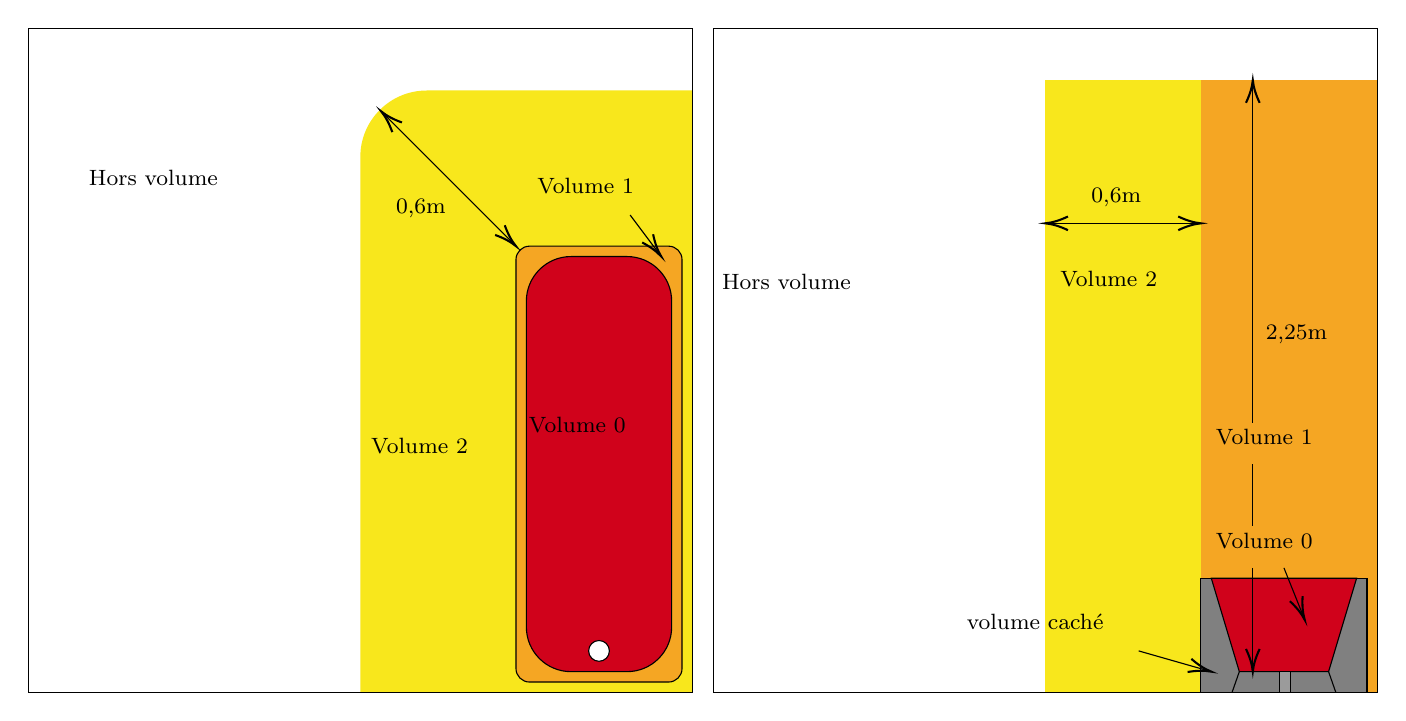
\begin{tikzpicture}[x=0.75pt,y=0.75pt,yscale=-1,xscale=1]
%uncomment if require: \path (0,550); %set diagram left start at 0, and has height of 550

%Shape: Rectangle [id:dp537465530048803] 
\draw  [draw opacity=0][fill={rgb, 255:red, 245; green, 166; blue, 35 }  ,fill opacity=1 ] (570,65) -- (655,65) -- (655,360) -- (570,360) -- cycle ;
%Rounded Single Corner Rect [id:dp9873012745251137] 
\draw  [draw opacity=0][fill={rgb, 255:red, 248; green, 231; blue, 28 }  ,fill opacity=1 ] (165,102) .. controls (165,84.33) and (179.33,70) .. (197,70) -- (325,70) -- (325,360) -- (165,360) -- cycle ;
%Rounded Rect [id:dp11224704269677876] 
\draw  [fill={rgb, 255:red, 245; green, 166; blue, 35 }  ,fill opacity=1 ] (240,151.5) .. controls (240,147.91) and (242.91,145) .. (246.5,145) -- (313.5,145) .. controls (317.09,145) and (320,147.91) .. (320,151.5) -- (320,348.5) .. controls (320,352.09) and (317.09,355) .. (313.5,355) -- (246.5,355) .. controls (242.91,355) and (240,352.09) .. (240,348.5) -- cycle ;
%Shape: Rectangle [id:dp6813821922304953] 
\draw  [draw opacity=0][fill={rgb, 255:red, 248; green, 231; blue, 28 }  ,fill opacity=1 ] (495,65) -- (570,65) -- (570,360) -- (495,360) -- cycle ;
%Straight Lines [id:da9776864357431949] 
\draw    (176.41,81.41) -- (238.59,143.59) ;
\draw [shift={(240,145)}, rotate = 225] [color={rgb, 255:red, 0; green, 0; blue, 0 }  ][line width=0.75]    (10.93,-3.29) .. controls (6.95,-1.4) and (3.31,-0.3) .. (0,0) .. controls (3.31,0.3) and (6.95,1.4) .. (10.93,3.29)   ;
\draw [shift={(175,80)}, rotate = 45] [color={rgb, 255:red, 0; green, 0; blue, 0 }  ][line width=0.75]    (10.93,-3.29) .. controls (6.95,-1.4) and (3.31,-0.3) .. (0,0) .. controls (3.31,0.3) and (6.95,1.4) .. (10.93,3.29)   ;
%Shape: Square [id:dp41030709608176064] 
\draw   (335,40) -- (655,40) -- (655,360) -- (335,360) -- cycle ;
%Shape: Square [id:dp14415595503059908] 
\draw   (5,40) -- (325,40) -- (325,360) -- (5,360) -- cycle ;
%Straight Lines [id:da04424757259652501] 
\draw    (295,130) -- (308.8,148.4) ;
\draw [shift={(310,150)}, rotate = 233.13] [color={rgb, 255:red, 0; green, 0; blue, 0 }  ][line width=0.75]    (10.93,-3.29) .. controls (6.95,-1.4) and (3.31,-0.3) .. (0,0) .. controls (3.31,0.3) and (6.95,1.4) .. (10.93,3.29)   ;
%Rounded Rect [id:dp9600049756918252] 
\draw  [fill={rgb, 255:red, 208; green, 2; blue, 27 }  ,fill opacity=1 ] (245,171.5) .. controls (245,159.63) and (254.63,150) .. (266.5,150) -- (293.5,150) .. controls (305.37,150) and (315,159.63) .. (315,171.5) -- (315,328.5) .. controls (315,340.37) and (305.37,350) .. (293.5,350) -- (266.5,350) .. controls (254.63,350) and (245,340.37) .. (245,328.5) -- cycle ;
%Shape: Circle [id:dp7093382716801047] 
\draw  [fill={rgb, 255:red, 255; green, 255; blue, 255 }  ,fill opacity=1 ] (275,340) .. controls (275,337.24) and (277.24,335) .. (280,335) .. controls (282.76,335) and (285,337.24) .. (285,340) .. controls (285,342.76) and (282.76,345) .. (280,345) .. controls (277.24,345) and (275,342.76) .. (275,340) -- cycle ;
%Shape: Rectangle [id:dp46214446507827656] 
\draw  [fill={rgb, 255:red, 128; green, 128; blue, 128 }  ,fill opacity=1 ] (570,305) -- (650,305) -- (650,360) -- (570,360) -- cycle ;
%Shape: Trapezoid [id:dp945587283320089] 
\draw  [fill={rgb, 255:red, 208; green, 2; blue, 27 }  ,fill opacity=1 ] (575,305) -- (588.5,350) -- (631.5,350) -- (645,305) -- cycle ;
%Straight Lines [id:da45767444398518653] 
\draw    (588.5,350) -- (585,360) ;
%Straight Lines [id:da303792904954273] 
\draw    (631.5,350) -- (635,360) ;
%Shape: Rectangle [id:dp35718485744867867] 
\draw  [fill={rgb, 255:red, 155; green, 155; blue, 155 }  ,fill opacity=1 ] (608,350) -- (613,350) -- (613,360) -- (608,360) -- cycle ;

%Straight Lines [id:da2781237207088538] 
\draw    (497,134) -- (568,134) ;
\draw [shift={(570,134)}, rotate = 180] [color={rgb, 255:red, 0; green, 0; blue, 0 }  ][line width=0.75]    (10.93,-3.29) .. controls (6.95,-1.4) and (3.31,-0.3) .. (0,0) .. controls (3.31,0.3) and (6.95,1.4) .. (10.93,3.29)   ;
\draw [shift={(495,134)}, rotate = 0] [color={rgb, 255:red, 0; green, 0; blue, 0 }  ][line width=0.75]    (10.93,-3.29) .. controls (6.95,-1.4) and (3.31,-0.3) .. (0,0) .. controls (3.31,0.3) and (6.95,1.4) .. (10.93,3.29)   ;
%Straight Lines [id:da9991563401347446] 
\draw    (595,300) -- (595,348) ;
\draw [shift={(595,350)}, rotate = 270] [color={rgb, 255:red, 0; green, 0; blue, 0 }  ][line width=0.75]    (10.93,-3.29) .. controls (6.95,-1.4) and (3.31,-0.3) .. (0,0) .. controls (3.31,0.3) and (6.95,1.4) .. (10.93,3.29)   ;
%Straight Lines [id:da9518092424958232] 
\draw    (595,67) -- (595,230) ;
\draw [shift={(595,65)}, rotate = 90] [color={rgb, 255:red, 0; green, 0; blue, 0 }  ][line width=0.75]    (10.93,-3.29) .. controls (6.95,-1.4) and (3.31,-0.3) .. (0,0) .. controls (3.31,0.3) and (6.95,1.4) .. (10.93,3.29)   ;
%Straight Lines [id:da21574516652189846] 
\draw    (595,250) -- (595,280) ;
%Straight Lines [id:da7442389799673409] 
\draw    (610,300) -- (619.26,323.14) ;
\draw [shift={(620,325)}, rotate = 248.2] [color={rgb, 255:red, 0; green, 0; blue, 0 }  ][line width=0.75]    (10.93,-3.29) .. controls (6.95,-1.4) and (3.31,-0.3) .. (0,0) .. controls (3.31,0.3) and (6.95,1.4) .. (10.93,3.29)   ;
%Straight Lines [id:da6922315454679567] 
\draw    (540,340) -- (573.08,349.45) ;
\draw [shift={(575,350)}, rotate = 195.95] [color={rgb, 255:red, 0; green, 0; blue, 0 }  ][line width=0.75]    (10.93,-3.29) .. controls (6.95,-1.4) and (3.31,-0.3) .. (0,0) .. controls (3.31,0.3) and (6.95,1.4) .. (10.93,3.29)   ;

% Text Node
\draw (501,156) node [anchor=north west][inner sep=0.75pt]   [align=left] {\footnotesize{Volume 2}};
% Text Node
\draw (576,232) node [anchor=north west][inner sep=0.75pt]   [align=left] {\footnotesize{Volume 1}};
% Text Node
\draw (169,236) node [anchor=north west][inner sep=0.75pt]   [align=left] {\footnotesize{Volume 2}};
% Text Node
\draw (249,111) node [anchor=north west][inner sep=0.75pt]   [align=left] {\footnotesize{Volume 1}};
% Text Node
\draw (338,157) node [anchor=north west][inner sep=0.75pt]   [align=left] {\footnotesize{Hors volume}};
% Text Node
\draw (33,107) node [anchor=north west][inner sep=0.75pt]   [align=left] {\footnotesize{Hors volume}};
% Text Node
\draw (245,226) node [anchor=north west][inner sep=0.75pt]   [align=left] {\footnotesize{Volume 0}};
% Text Node
\draw (181,121) node [anchor=north west][inner sep=0.75pt]   [align=left] {\footnotesize{0,6m}};
% Text Node
\draw (576,282) node [anchor=north west][inner sep=0.75pt]   [align=left] {\footnotesize{Volume 0}};
% Text Node
\draw (516,116) node [anchor=north west][inner sep=0.75pt]   [align=left] {\footnotesize{0,6m}};
% Text Node
\draw (600,182) node [anchor=north west][inner sep=0.75pt]   [align=left] {\footnotesize{2,25m}};
% Text Node
\draw (456,321) node [anchor=north west][inner sep=0.75pt]   [align=left] {\footnotesize{volume caché}};


\end{tikzpicture}

\end{figure}




%\end{document}

